\documentclass[letterpaper, 12pt]{article}
\usepackage{pdfpages}

\usepackage{geometry}
 \geometry{
 letterpaper,
 total={170mm,257mm},
 left=20mm,
 top=20mm,
 bottom=20mm
 }
\usepackage{graphicx} % Required for inserting images
\usepackage{authblk}
\usepackage{amssymb}
\usepackage{lipsum}
\usepackage{float}
\usepackage{times}
\usepackage{amsmath}
\usepackage[format=plain,
            labelfont={bf,it},
            textfont=it]{caption}
\captionsetup{justification=raggedright,singlelinecheck=false}
\usepackage{ragged2e}
\usepackage{longtable}
\usepackage{comment}
\usepackage{setspace}
\usepackage{fancyhdr}
\usepackage{titlesec}
\usepackage[hyperindex,breaklinks]{hyperref}
\hypersetup{
    colorlinks=true,
    linkcolor=blue,
    filecolor=magenta,      
    urlcolor=blue,
    pdftitle={Overleaf Example},
    pdfpagemode=FullScreen,
    }
% \usepackage{background} % add COSIG logo to page
\usepackage[T1]{fontenc}
\usepackage{helvet}
\renewcommand{\familydefault}{\sfdefault}
\pagenumbering{gobble}
\usepackage[skip=10pt plus1pt, indent=40pt]{parskip}

\begin{comment}
\backgroundsetup{
   scale=1,
   angle=0,
   opacity=1,
   color=black,
   contents={\begin{tikzpicture}[remember picture, overlay]
      \node at ([xshift=3cm,yshift=1cm] current page.south west)
            {
\includegraphics[width = 5cm]{img/home/241017_final_logo_mockup.png}}; %<- change the name of image
     \end{tikzpicture}}
 }
\end{comment}

\titlespacing*{\section}
{0pt}{1.5ex plus 1ex minus .2ex}{1.3ex plus .2ex}

\renewcommand\Authfont{\fontsize{12}{14.4}\selectfont}
\renewcommand\Affilfont{\fontsize{9}{10.8}\itshape}


\begin{document}


\includepdf[pages=-]{pdfs/cosig_home.pdf}\label{g:cosig_home}

\includepdf[pages=-]{pdfs/cell_lines.pdf}\label{g:cell_lines}
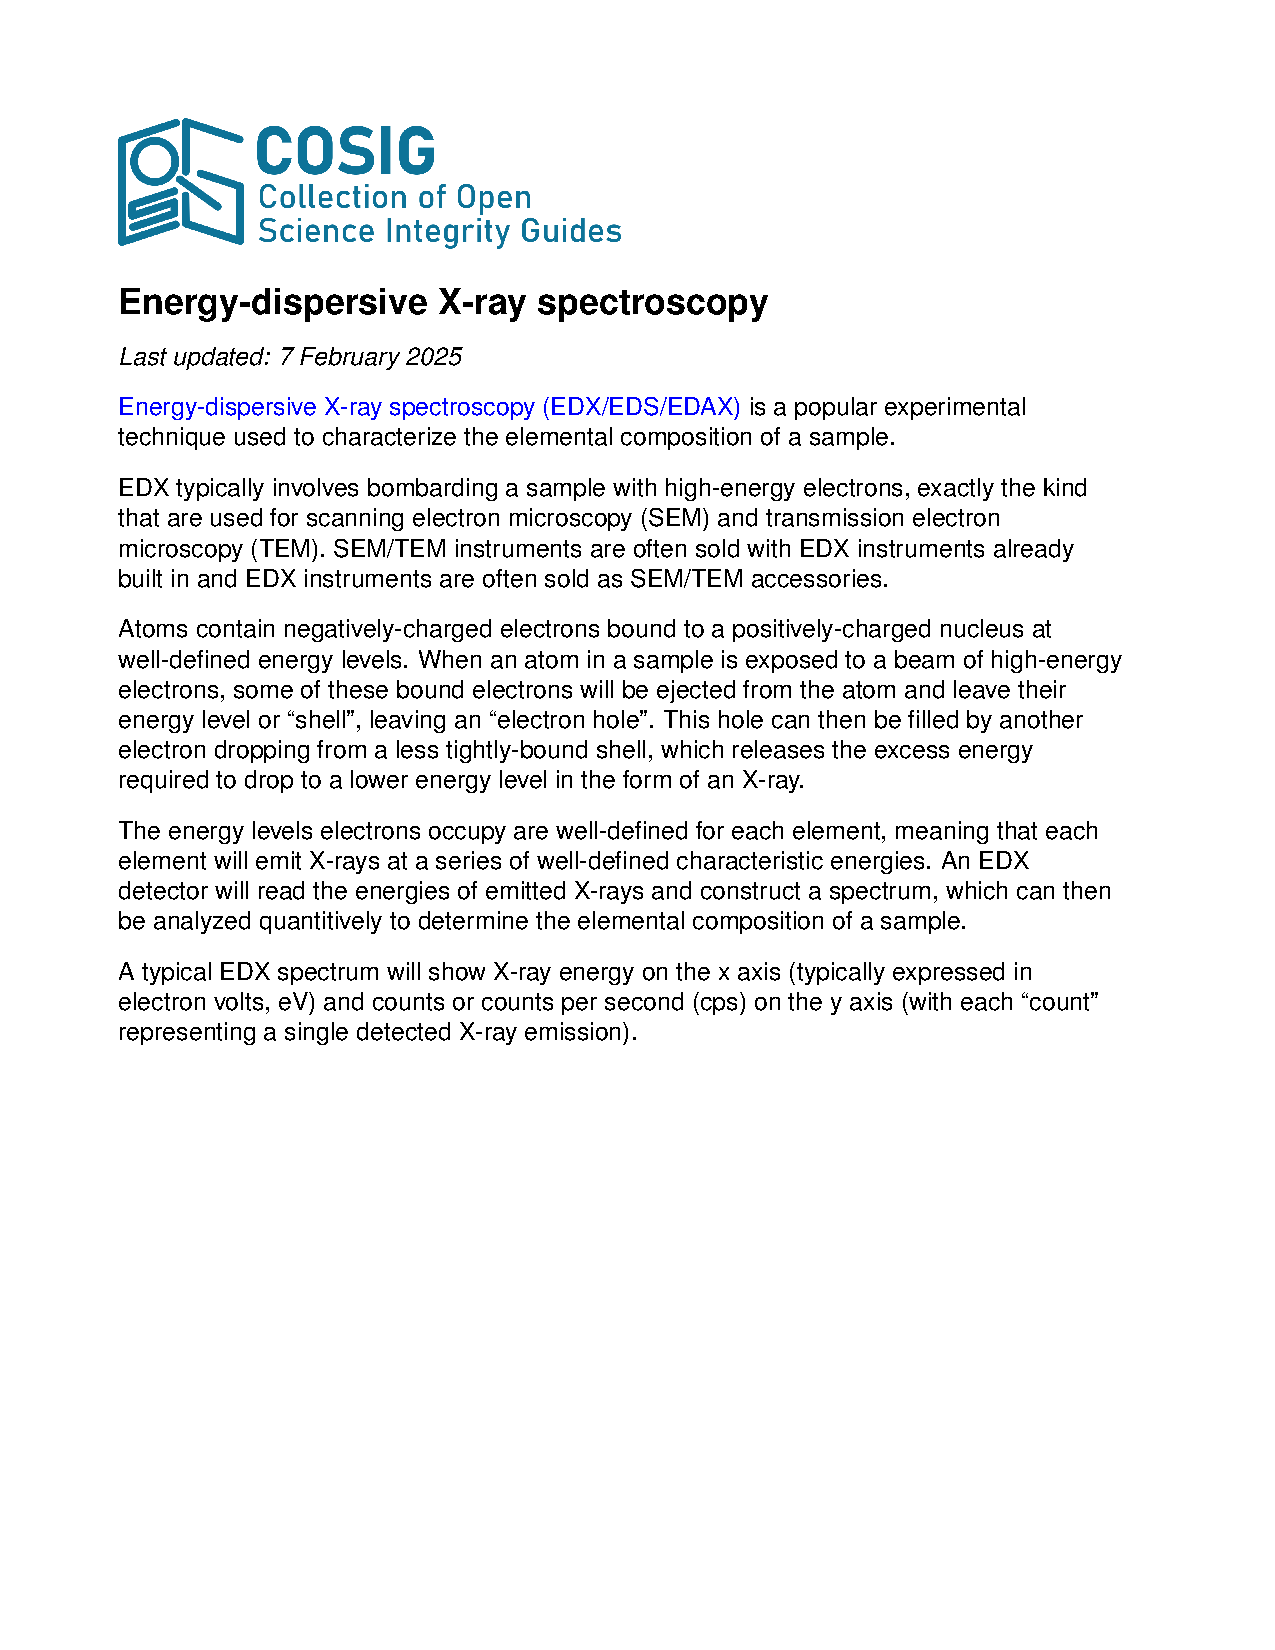
\includepdf[pages=-]{pdfs/edx.pdf}\label{g:edx}

\includepdf[pages=-]{pdfs/pubpeer_best_practices.pdf}\label{pubpeer_best_practices}
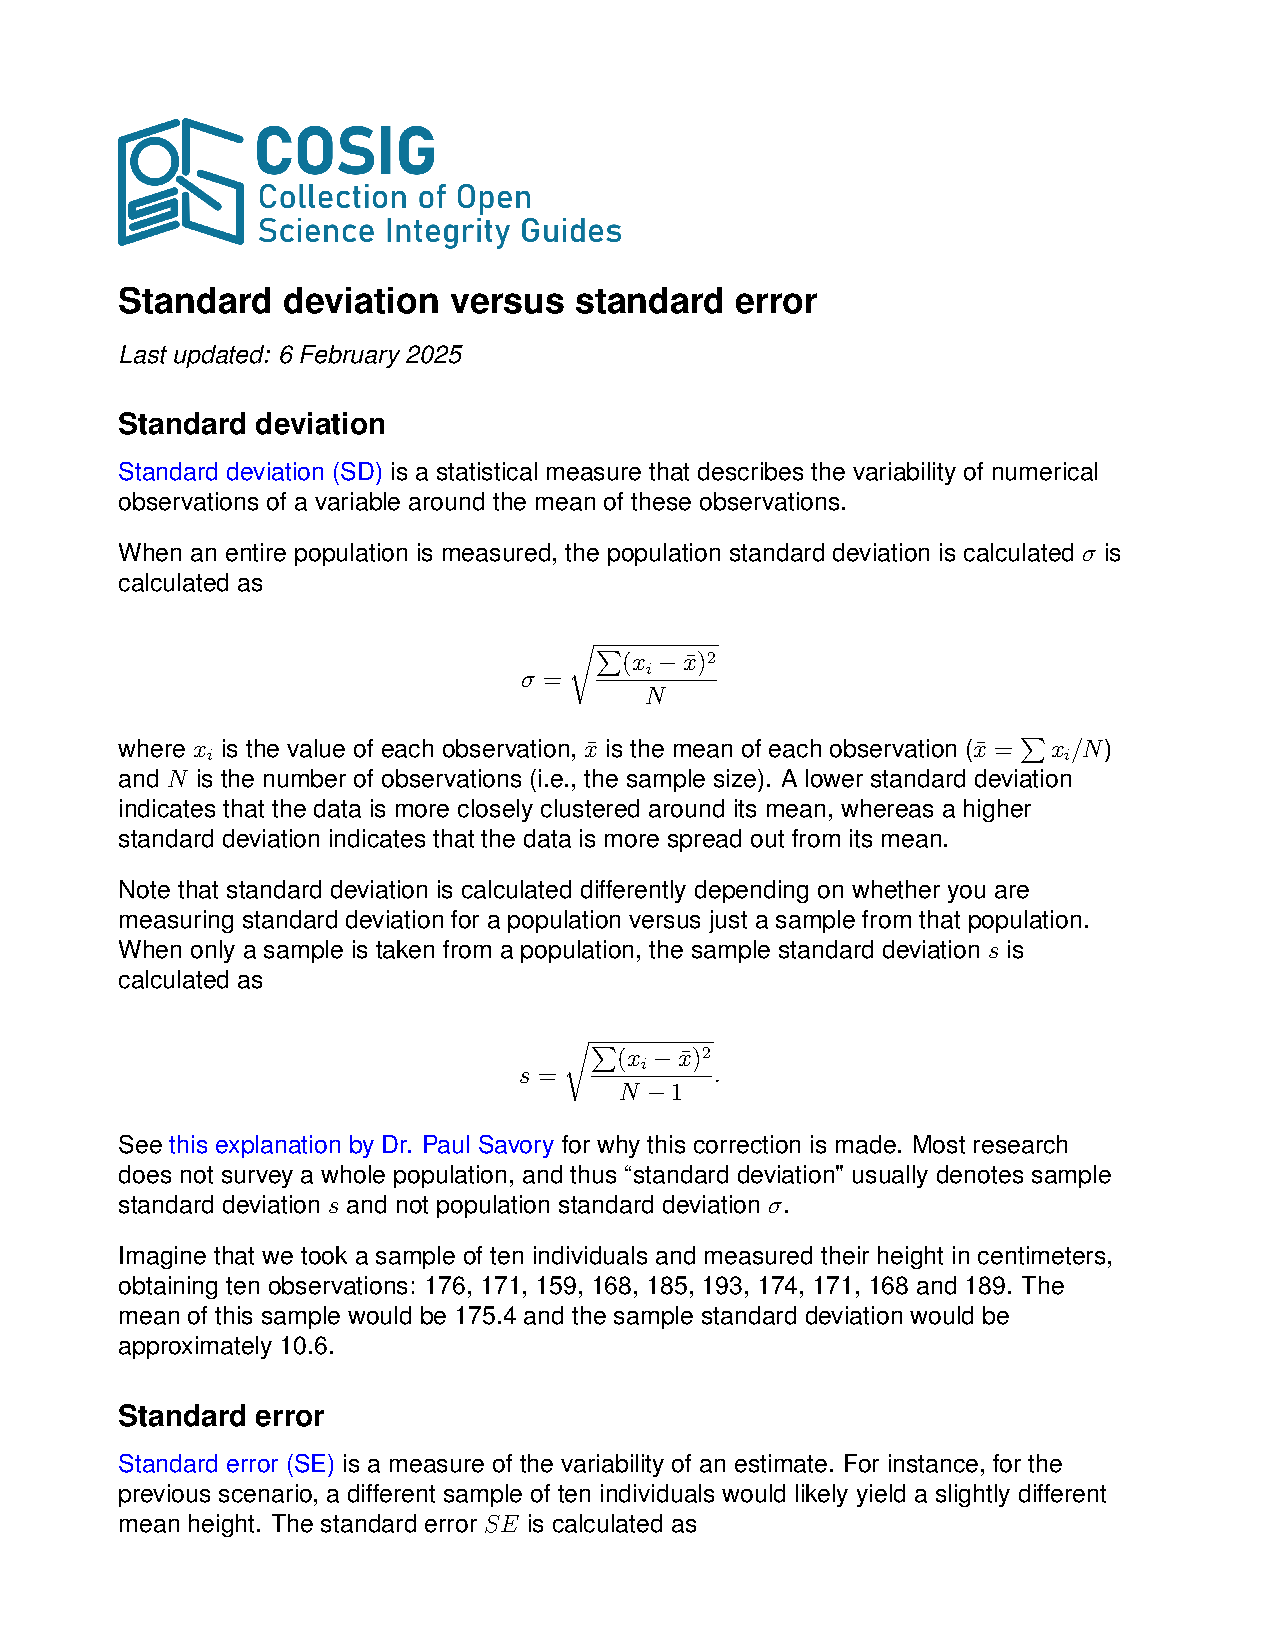
\includepdf[pages=-]{pdfs/sd_vs_se.pdf}\label{g:sd_vs_se}
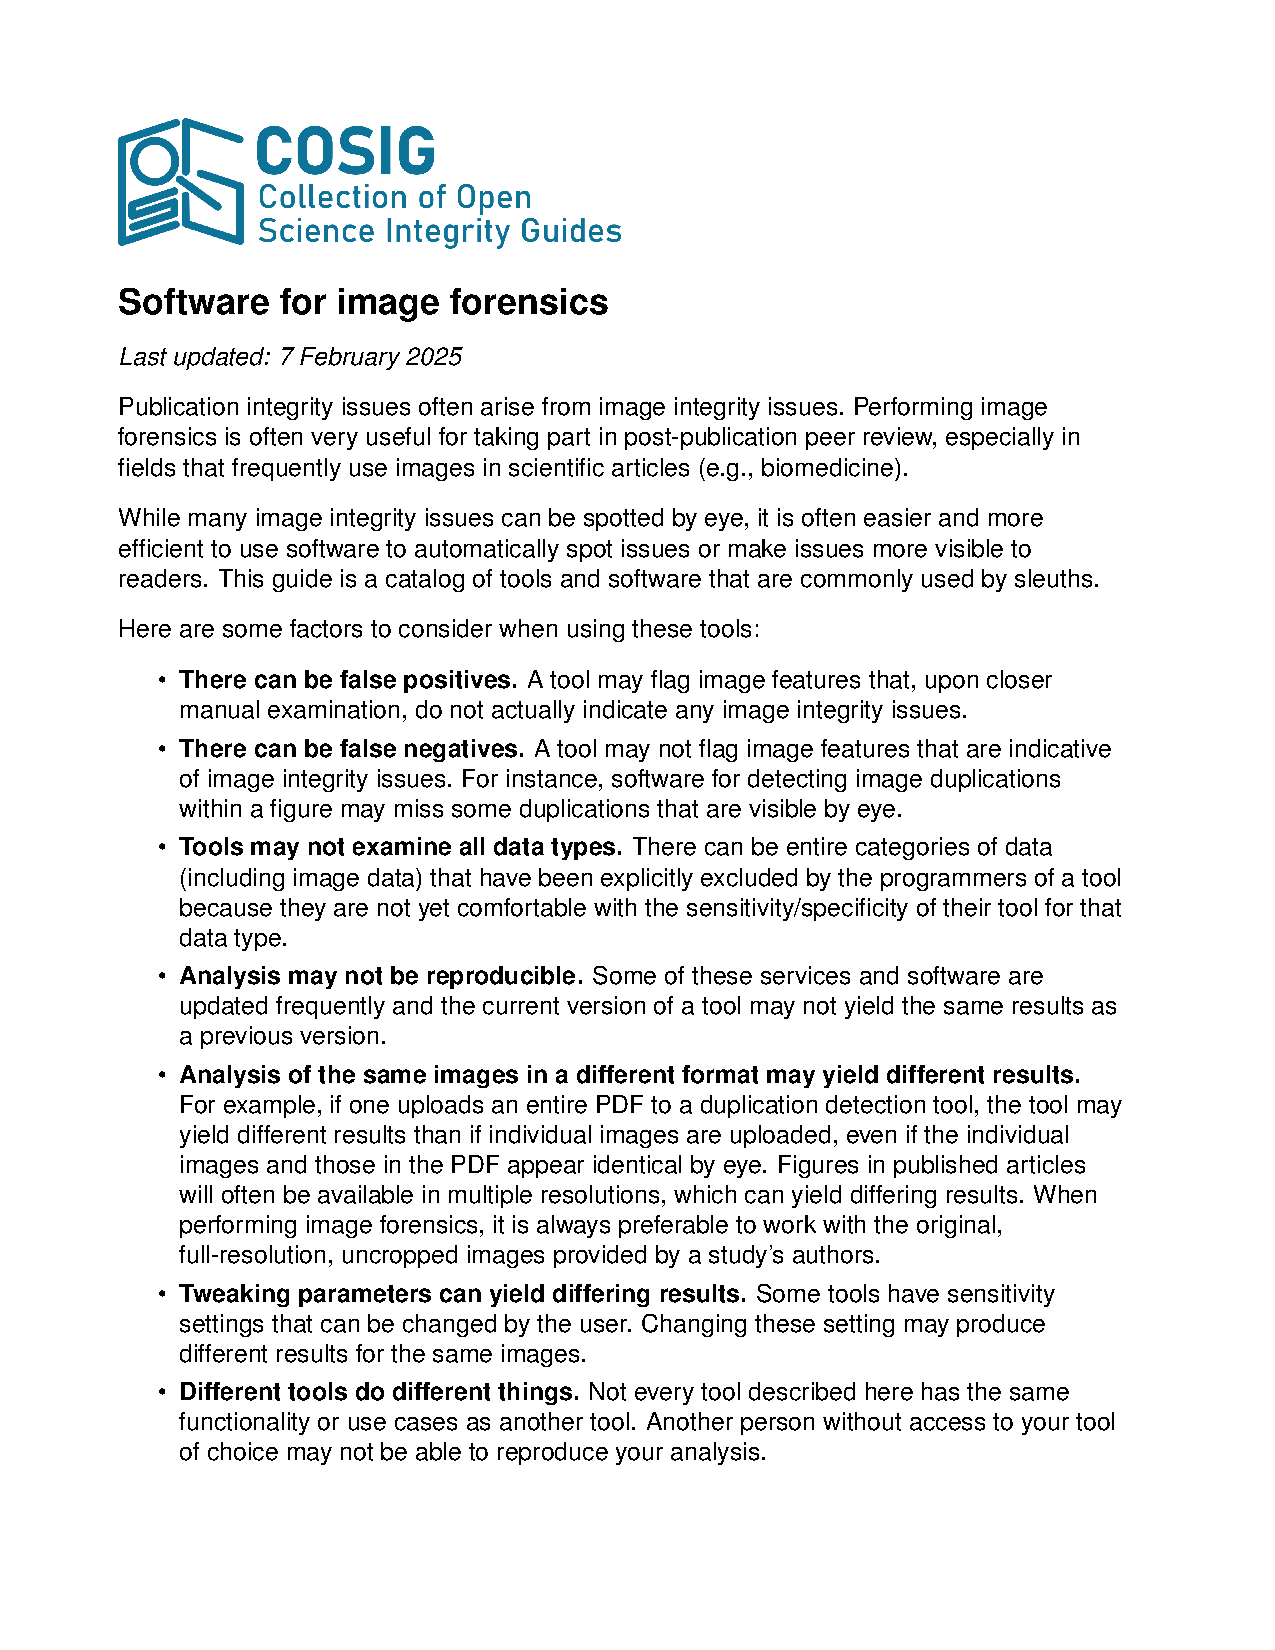
\includepdf[pages=-]{pdfs/software_image_forensics.pdf}\label{g:software_image_forensics}
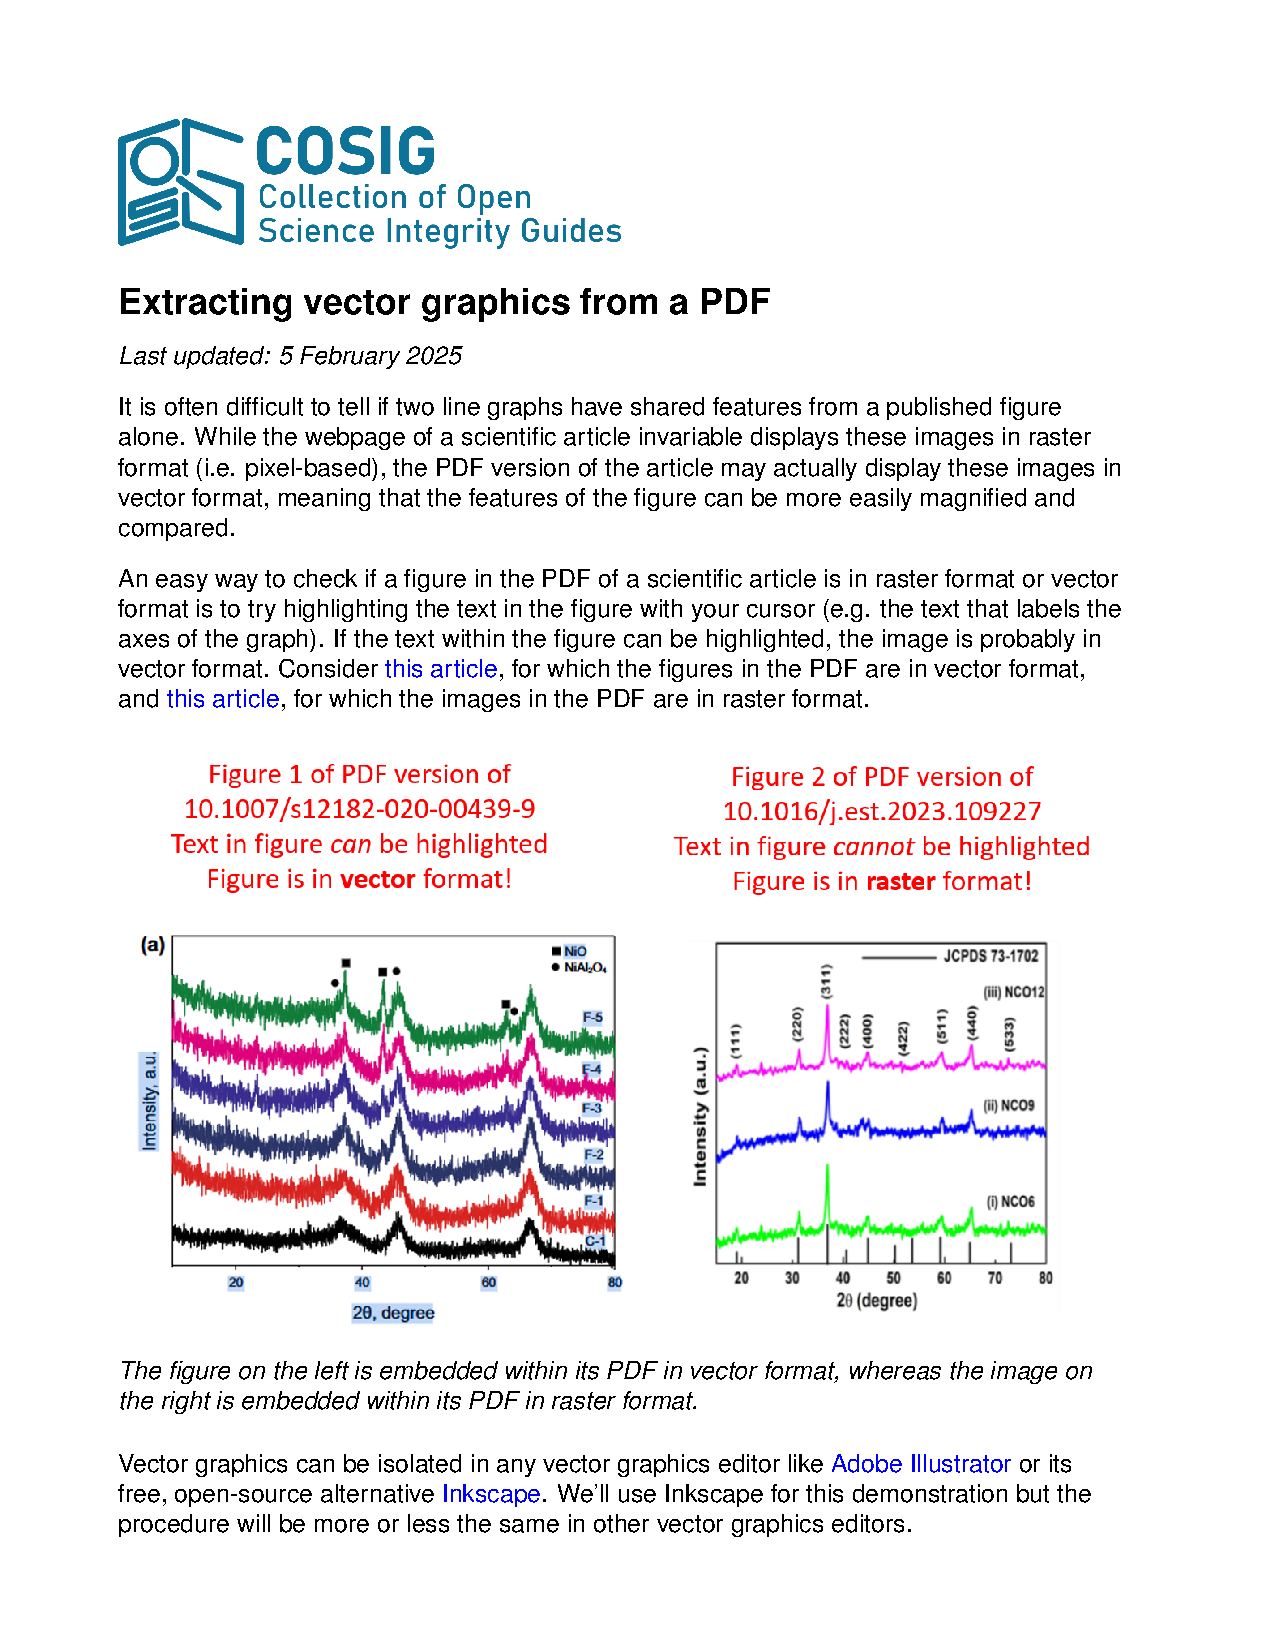
\includepdf[pages=-]{pdfs/vector_graphics.pdf}\label{g:vector_graphics}
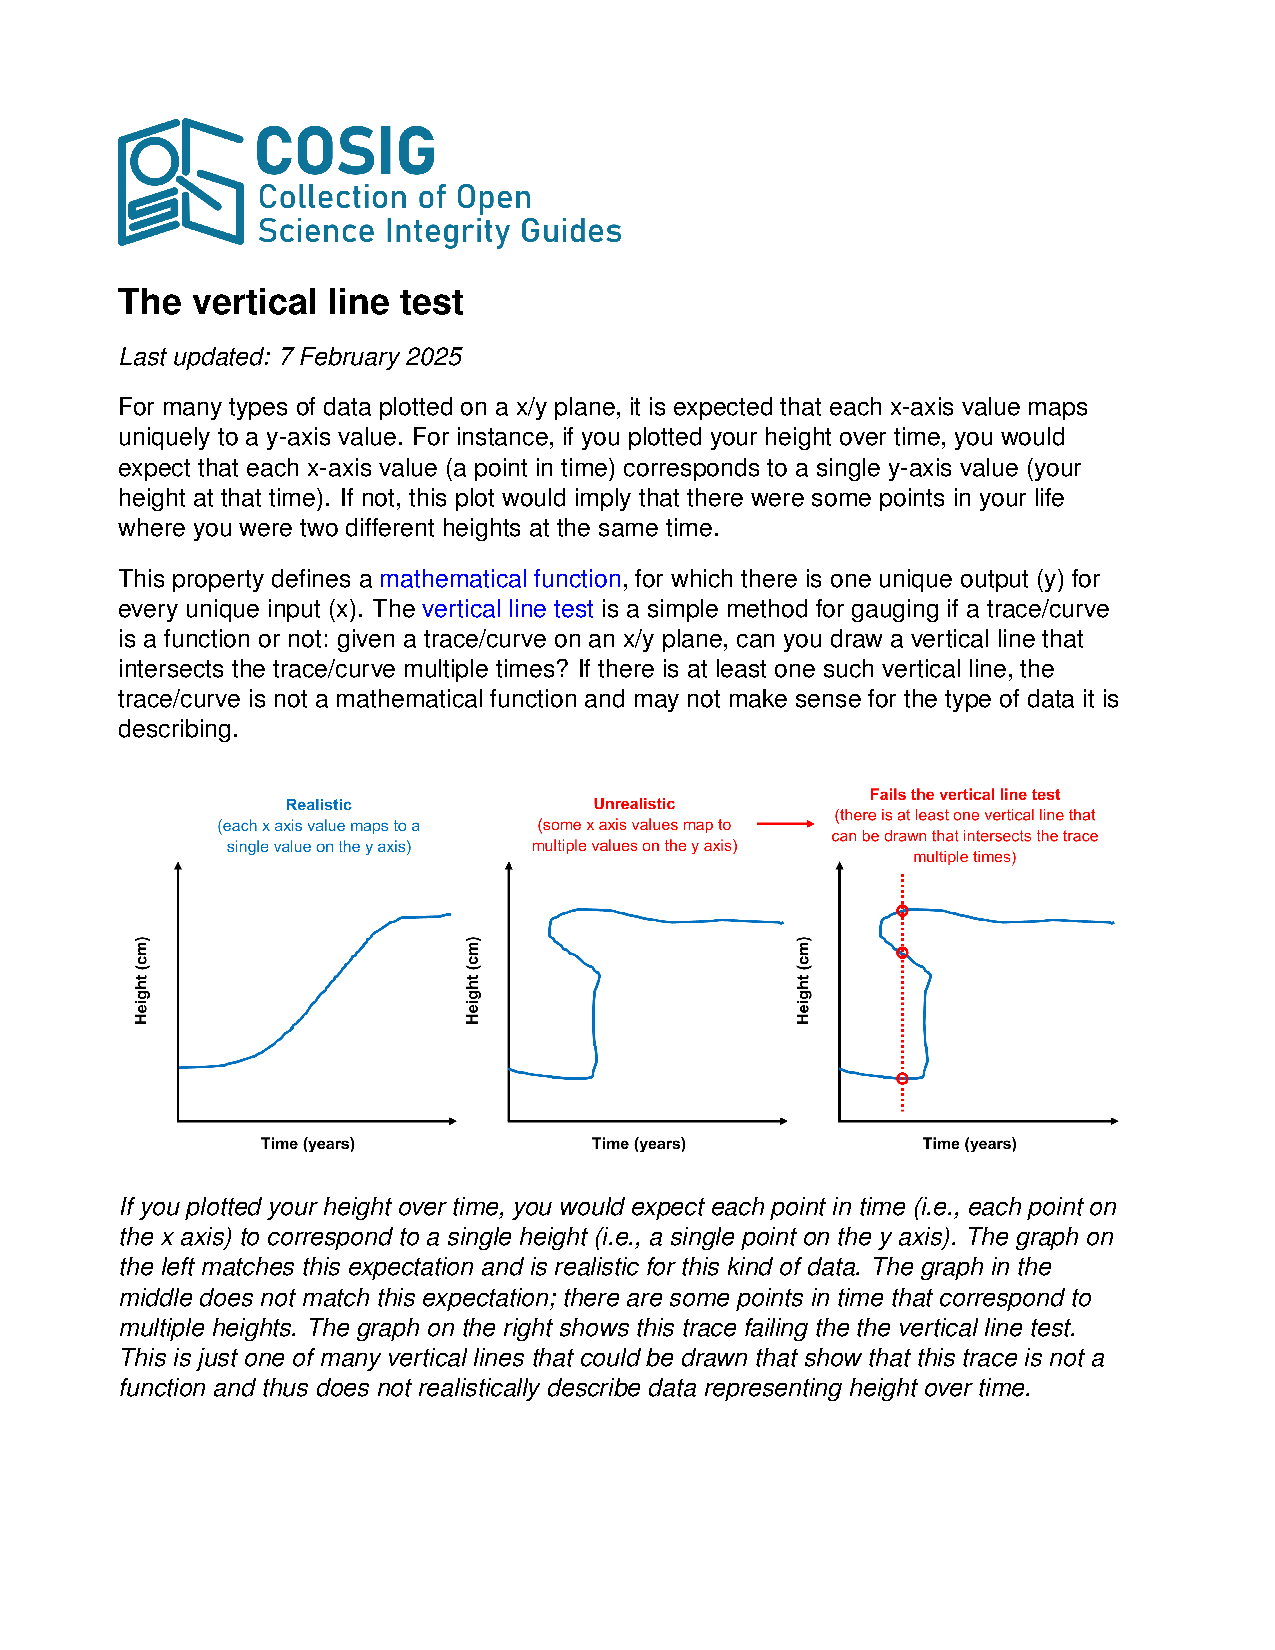
\includepdf[pages=-]{pdfs/vertical_line.pdf}\label{g:vertical_line}
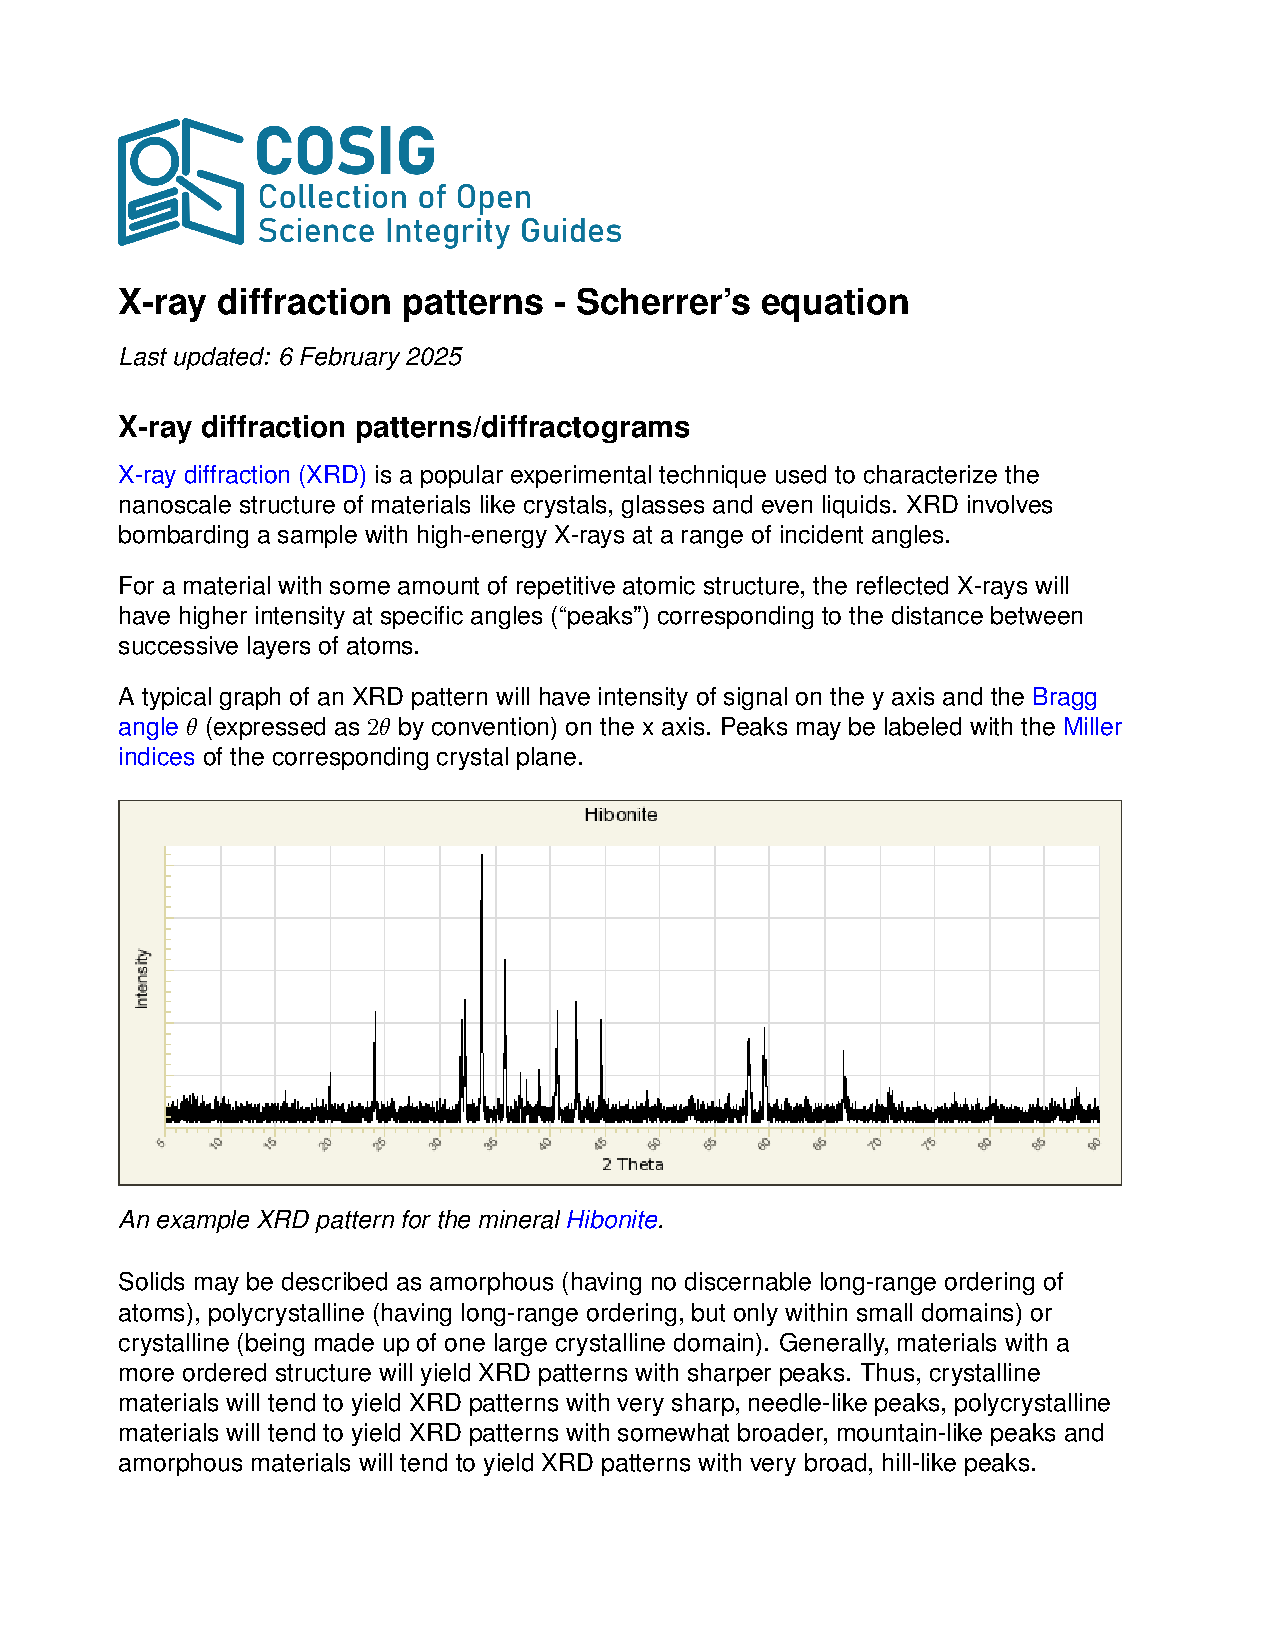
\includepdf[pages=-]{pdfs/xrd_scherrer.pdf}\label{xrd_scherrer}

\end{document}